\documentclass[a4paper]{article}
\usepackage{mystyle}

\begin{document}

\customtitle{Fluctuation Strength Model Implementation}

\section{Introduction}

The following document details the implementation of a fluctuation strength
model, based on the roughness model implemented by \citet{Schrader2002}.
This is similar to the work of \citet{Sontacchi1998}, which will be also
taken into account when making the necessary adjustments.

First the model will be implemented for AM (amplitude-modulated) tones; later it
will be extended to cover also FM (frequency-modulated) tones and AM BBN
(broadband noise).

In order to validate the implemented model with the data available on literature
(e.g., \citet{Fastl2007Psychoacoustics}), several values and plots will be
specified. These will determine the expected output from the model, and will
serve to confirm the correctness of the implementation.

\section{Implementation}

The following are implementation details of the roughness model that probably
will have to be adjusted for the fluctuation strength model.

\begin{itemize}
    \item Does the FFT resolution affects in any way the results of the model?
    \item \matlabinline{Hweight} models the bandpass response of the modulation
        frequency, do these weights have to be changed for the fluctuation
        strength case?
    \item \matlabinline{gzi} represents the effect of the carrier frequency on
        the output, do these values have to be changed for the fluctuation
        strength case?
    \item Does the relation $f_s \propto m_d ^ 2$ still holds?
\end{itemize}

\subsection{FFT Resolution}

\subsection{Modulation Frequency Dependency}

\subsection{Carrier Frequency Dependency}

Regarding carrier frequency, a difference exists whether the signal is an AM
tone or an FM tone. This can be appreciated in Figure
\ref{fig:flucstrenvscfreq}. This is a detail to consider when modeling the
carrier frequency effect on fluctuation strength.

\begin{figure}[ht]
    \centering
    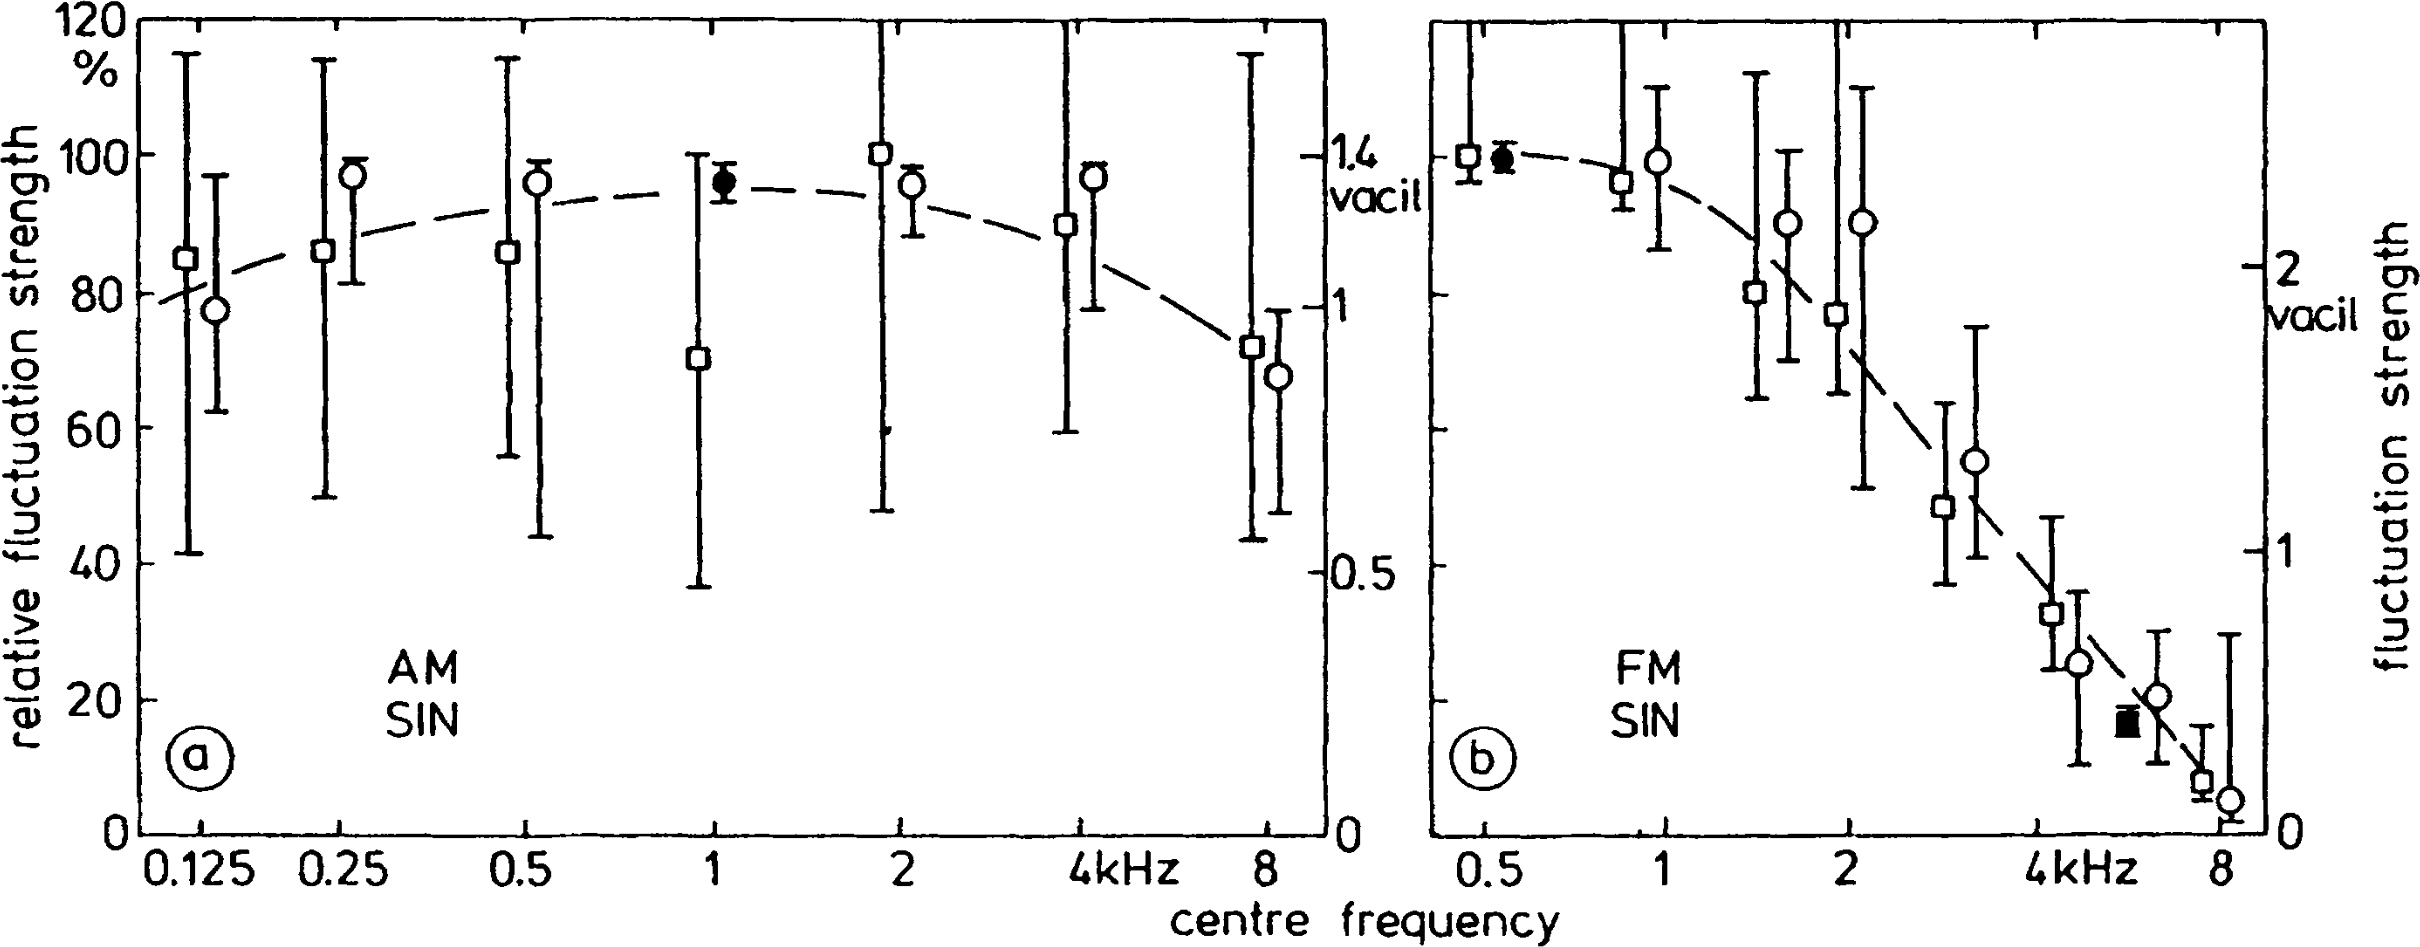
\includegraphics[height=5cm]
        {book/img/Fastl2007-FluctuationStrengthVsCenterFrequency}
    \caption{Fluctuation strength as a function of center frequency
        \cite[pp. 250]{Fastl2007Psychoacoustics}}
    \label{fig:flucstrenvscfreq}
\end{figure}

\subsection{Modulation Depth Dependency}

In the model by \citet{Sontacchi1998} the exponent $2$ is used in the modulation
depth relation; this based on the roughness models of
\citet{aures1985berechnungsverfahren} and \citet{daniel1997psychoacoustical}.
However, it is to note that the relation between modulation depth and
fluctuation strength is not that straightforward as in roughness. This can be
appreciated in Figure \ref{fig:flucstrenvsmoddep}, where it can be seen that for
AM tones only between 4 and 20 dB the relation is somewhat linear. This
contrasts with the case of roughness, depicted in Figure \ref{fig:roughdegmod}.
As so, it is to consider whether the used relation is representative for the
fluctuation strength case.

\begin{figure}[ht]
    \centering
    \begin{minipage}[b]{0.45\linewidth}
        \centering
        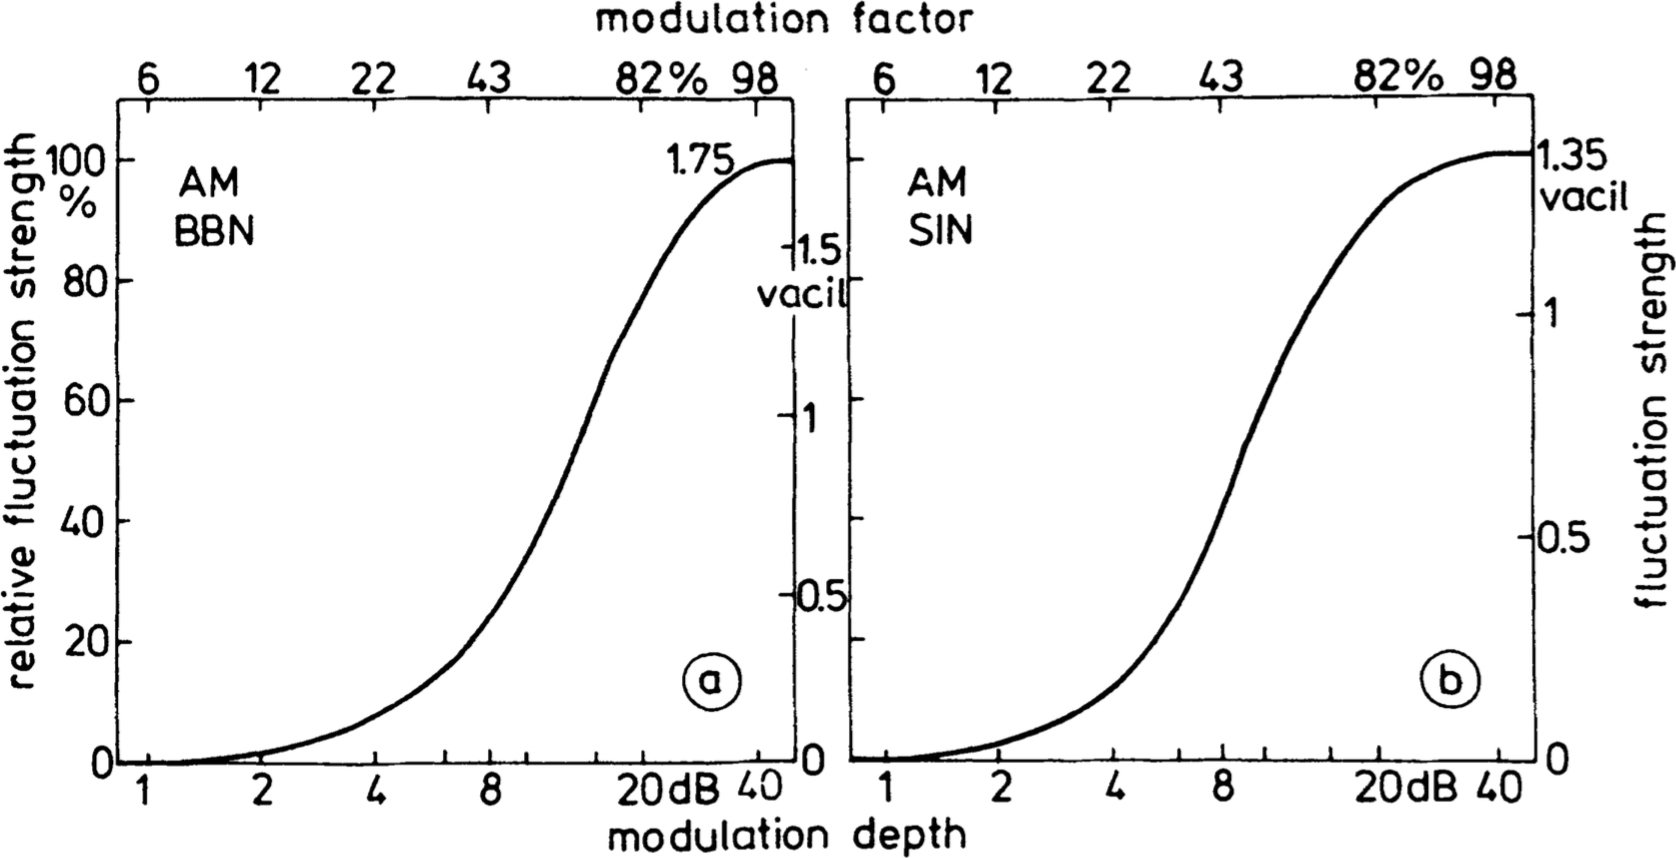
\includegraphics[height=3.5cm]
            {book/img/Fastl2007-FluctuationStrengthVsModulationDepth}
        \caption{Fluctuation strength as a function of modulation depth
            \cite[pp. 249]{Fastl2007Psychoacoustics}}
        \label{fig:flucstrenvsmoddep}
    \end{minipage}
    \quad
    \begin{minipage}[b]{0.45\linewidth}
        \centering
        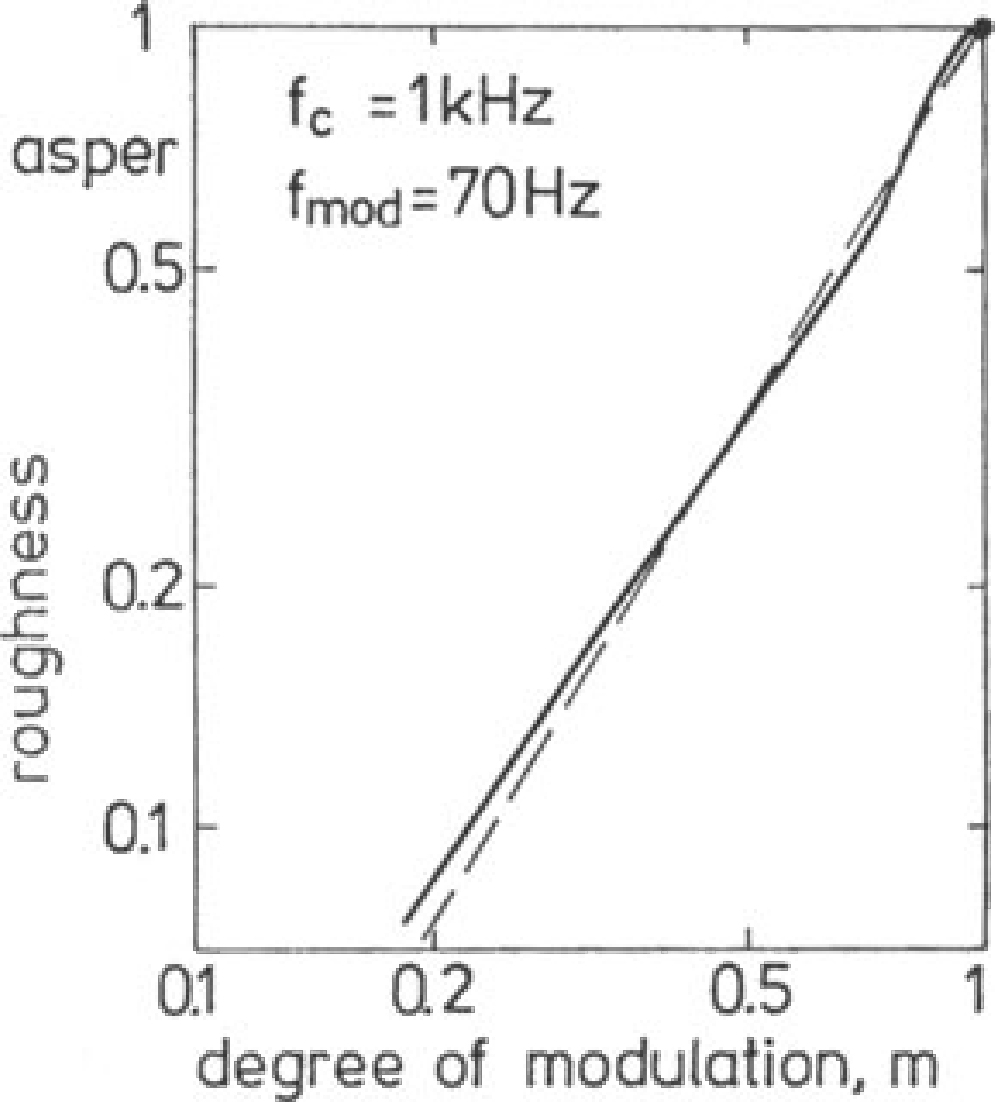
\includegraphics[height=3.5cm]
            {book/img/Fastl2007-RoughnessDegreeModulation}
        \caption{Roughness as a function of degree of modulation
            \cite[pp. 258]{Fastl2007Psychoacoustics}}
        \label{fig:roughdegmod}
    \end{minipage}
\end{figure}

\bibliographystyle{plainnat}
\bibliography{../References}

\end{document}
